% Self-contained source: no external figures, bibliography database, or app required.
% Build: latexmk -pdf graphmine.tex
% Alternative: tectonic graphmine.tex
% With pdflatex alone, run it twice to resolve the contents and references.
\documentclass[11pt,a4paper]{article}
\usepackage[T1]{fontenc}
\usepackage{iftex}
\ifPDFTeX
  \usepackage[utf8]{inputenc}
\fi
\usepackage{lmodern}
\usepackage[margin=25mm]{geometry}
\usepackage{microtype}
\usepackage{amsmath,amssymb}
\usepackage{booktabs,tabularx,longtable,array}
\usepackage{graphicx}
\usepackage{xcolor}
\usepackage{tikz}
\usetikzlibrary{arrows.meta,positioning,fit,backgrounds}
\usepackage{listings}
\usepackage{enumitem}
\usepackage{xurl}
\usepackage[colorlinks=true,linkcolor=teal!65!black,citecolor=teal!65!black,
  urlcolor=teal!65!black,pdftitle={GraphMine: From Business Questions to Auditable GPU Graph Analysis}]{hyperref}
\usepackage{bookmark}

\definecolor{ink}{HTML}{173047}
\definecolor{accent}{HTML}{167D8D}
\definecolor{pale}{HTML}{EDF6F7}
\definecolor{warm}{HTML}{FFF4DF}
\setlength{\parindent}{0pt}
\setlength{\parskip}{0.55em}
\setlength{\emergencystretch}{2em}
\setcounter{tocdepth}{2}
\setlist{itemsep=0.2em,topsep=0.3em}
\newcolumntype{Y}{>{\raggedright\arraybackslash}X}
\newcolumntype{P}[1]{>{\raggedright\arraybackslash}p{#1}}
\newcommand{\code}[1]{\texttt{\detokenize{#1}}}
\newcommand{\pathref}[1]{\nolinkurl{#1}}
\newcommand{\intuition}[1]{\par\textbf{Intuition.} #1\par}
\newcommand{\technical}[1]{\par\textbf{Technical view.} #1\par}
\lstset{basicstyle=\ttfamily\small,breaklines=true,columns=fullflexible,
  keepspaces=true,showstringspaces=false,frame=single,
  rulecolor=\color{accent!35},backgroundcolor=\color{pale},
  xleftmargin=0.5em,xrightmargin=0.5em,aboveskip=0.8em,belowskip=0.8em}
\tikzset{box/.style={draw=accent!75,rounded corners=3pt,fill=pale,
  align=center,font=\small,inner sep=7pt},
  gate/.style={box,fill=warm,draw=orange!60!black},
  arrow/.style={-{Latex[length=2mm]},thick,draw=ink}}

\title{\vspace{-1em}\textbf{\textcolor{ink}{GraphMine}}\\[0.4em]
  \Large From Business Questions to Auditable GPU Graph Analysis\\[0.6em]
  \large An intuition-first account of the architecture, training,\\
  evaluation, and feedback workflow}
\author{Project technical note}
\date{Implementation and experiment snapshot: October 2026\\
  \small Includes records from 1--4 October 2026 UTC}

\begin{document}
\maketitle

\begin{abstract}
GraphMine lets a user ask practical questions about connected records without
having to name a graph algorithm or a GPU implementation. A language model
interprets the question, a deterministic application checks the proposed
analysis, a precompiled C++/CUDA library computes the result, and the application
turns that result into named records, tables, explanations, and visualizations.
This note explains that design from intuition to implementation. It also
describes the two completed local routing-adapter training runs and the business
question curriculum used by the current pilot. On 124 authored business routing
cases, the matched NF4 base passed 113 and the business adapter passed 118 under
the recorded application-aware review. This is limited routing evidence: the
review was refined during development, a grouping regression remains, and a
general improvement in complete user workflows has not been established.
The paper therefore separates working software, completed training, measured
results, and proposed next steps. The installed pilot is currently stopped at
the user's request; its weights and saved data are preserved.
\end{abstract}

\textbf{How to read this note.} Part I develops the idea with an ordinary staffing
question. Part II follows that question through the software. Part III explains
what was trained, how it was tested, and what the numbers mean. Part IV describes
the user-testing loop and the work still needed. The appendices identify the
source files, experiment records, and commands needed to revisit the system.

\clearpage
\begingroup
\small
\setlength{\parskip}{0pt}
\tableofcontents
\endgroup
\clearpage

\part{The idea, before the machinery}

\section{The problem GraphMine is trying to solve}

A project manager might ask, ``Which existing groups could work together on a
new project?'' An investigator might ask for mutually connected accounts to put
in a review queue. A researcher might want groups of associated proteins for
follow-up experiments. Each question combines a practical goal with a structural
question about relationships.

The user usually knows what a record means: an employee, an account, a device,
a product, or a protein. They may also know what an edge means: collaboration,
payment, communication, purchase, or association. They should not have to know
which implementation accepts those records, which parameters are semantic,
or which GPU backend was compiled.

GraphMine supplies the bridge between those two levels. It asks for a meaningful
business choice when the goal is unclear, translates a sufficiently precise
request into a supported computation, runs that computation, and explains the
returned evidence using the original records. For example, a good clarification
to ``Who should I focus on?'' asks whether the user wants people who connect
otherwise separate teams or people who have worked with many colleagues.
That distinction is useful to the user even without naming a centrality measure.

The current system is a graph-analysis application over uploaded data. Its
persistent store keeps conversations, files, jobs, results, and review evidence.
It does not establish that every business objective can be answered from graph
structure. A payment circle is a pattern in the records; deciding whether it is
fraud requires evidence outside that pattern.

\section{A running example: finding teams}
\label{sec:example}

Imagine a small collaboration dataset with five employees: Amina, Ben, Chen,
Dina, and Eli. Amina, Ben, Chen, and Dina have all worked with one another. Eli
has worked with Amina and Ben, but not with Chen or Dina. This is an illustrative
example for explaining semantics, not an additional measured experiment.

Suppose the user asks:
\begin{quote}
Help me staff projects with existing teams. Show every team of at least three
coworkers who have all worked with one another. Leave out a team if it is
entirely included in a larger qualifying team, and give me the members' names.
\end{quote}

There are two requested groups: \{Amina, Ben, Chen, Dina\} and
\{Amina, Ben, Eli\}. The smaller triplets inside the four-person group are not
separate answers because the request explicitly excludes them.

\intuition{The important work is preserving what ``every team'' means. Asking
for all complete groups, the largest complete group, or every three-person group
can produce different correct answers from exactly the same data.}

\technical{Represent the collaboration data as an undirected graph
$G=(V,E)$. A subset $C\subseteq V$ is a clique if every distinct pair in $C$ is
an edge. The request asks for all inclusion-maximal cliques with $|C|\geq 3$.}

Formally, the output family is
\begin{equation}
\mathcal{C}_{\mathrm{maximal}}=
\left\{C\subseteq V:
|C|\geq 3,\ \binom{C}{2}\subseteq E,\
\nexists v\in V\setminus C\text{ with }\binom{C\cup\{v\}}{2}\subseteq E
\right\}.
\end{equation}
Here $\binom{C}{2}$ means the set of unordered pairs of members of $C$.
``Maximal'' means a group cannot be extended; ``maximum'' means a group has the
largest possible size. If the user instead requests every three-person group,
including groups inside larger ones, the four-person clique contributes
$\binom{4}{3}=4$ triplets and Eli's group contributes one more. Returning only
the two full groups would answer a different question.

This distinction is also a real limitation of the pilot: a business-adapter
route confused exact-size payment groups with full groups in one saved
comparison. Section~\ref{sec:regression} explains how that mistake propagated.

\section{The central design: interpretation, computation, and evidence}

\intuition{Think of the system as an analyst using a tested analysis toolkit.
The analyst identifies the question and explains the answer. The toolkit performs
the calculation. A supervisor checks that the requested tool and its inputs are
allowed and that the answer can be traced back to the calculation.}

In GraphMine, the language model fills the interpretation role. The native
library supplies graph algorithms. The application performs validation,
orchestration, record joins, storage, and presentation. These components have
different responsibilities and fail in different ways:

\begin{itemize}
\item A router can choose the wrong mathematical problem even when its JSON is valid.
\item A planner can choose an invalid parameter or overlook a required input.
\item A native implementation can be incorrect or unsuitable for an input; the
  project therefore exposes implementations that passed its recorded validation.
\item A correct numerical result can still be presented badly, with missing
  names, an unreadable chart, or a claim stronger than the evidence.
\end{itemize}

This separation makes diagnosis possible. Improving the interface, fixing a
filter, and fine-tuning a router are three different changes. A better screen
does not demonstrate better model weights. A lower training loss does not show
that the user received the correct teams.

\part{How the application works}

\section{Architecture and the boundary around execution}
\label{sec:architecture}

The installed pilot has a browser application, a FastAPI service, two model
services, a serial native-job worker, and persistent storage. Figure~\ref{fig:arch}
shows their main relationships. The browser can run on another computer on the
private network; the application and model processes run on the GPU server.

\begin{figure}[htbp]
\centering
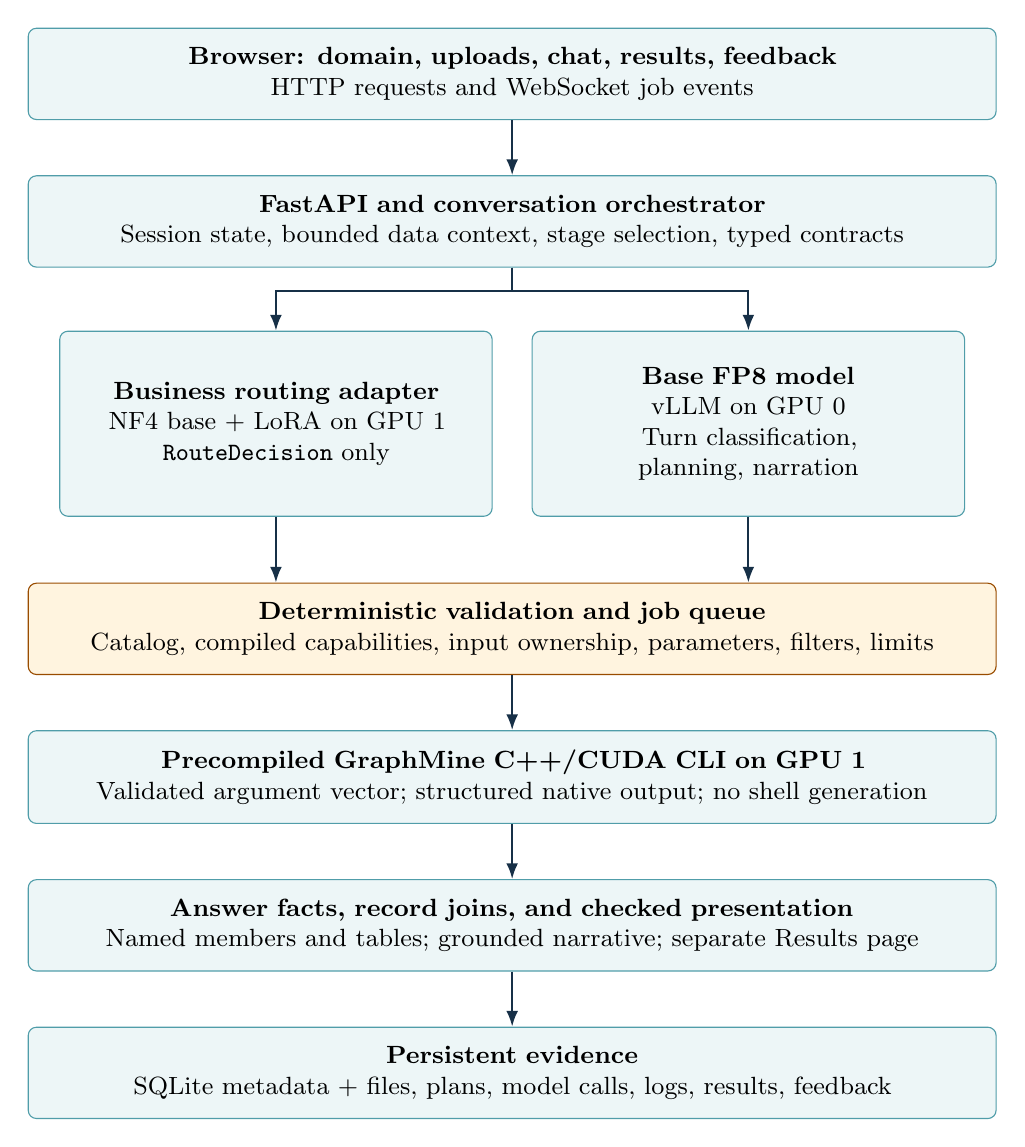
\begin{tikzpicture}[node distance=7mm]
\node[box,text width=11.8cm] (ui) {\textbf{Browser: domain, uploads, chat, results, feedback}\\
HTTP requests and WebSocket job events};
\node[box,text width=11.8cm,below=of ui] (api) {\textbf{FastAPI and conversation orchestrator}\\
Session state, bounded data context, stage selection, typed contracts};
\node[box,text width=5.0cm,minimum height=2.35cm,anchor=north] (route)
at ([xshift=-3cm,yshift=-8mm]api.south)
{\textbf{Business routing adapter}\\NF4 base + LoRA on GPU 1\\\code{RouteDecision} only};
\node[box,text width=5.0cm,minimum height=2.35cm,anchor=north] (base)
at ([xshift=3cm,yshift=-8mm]api.south)
{\textbf{Base FP8 model}\\vLLM on GPU 0\\Turn classification, planning, narration};
\node[gate,text width=11.8cm,below=40mm of api] (validate)
{\textbf{Deterministic validation and job queue}\\Catalog, compiled capabilities, input ownership, parameters, filters, limits};
\node[box,text width=11.8cm,below=of validate] (native)
{\textbf{Precompiled GraphMine C++/CUDA CLI on GPU 1}\\Validated argument vector; structured native output; no shell generation};
\node[box,text width=11.8cm,below=of native] (facts)
{\textbf{Answer facts, record joins, and checked presentation}\\Named members and tables; grounded narrative; separate Results page};
\node[box,text width=11.8cm,below=of facts] (store)
{\textbf{Persistent evidence}\\SQLite metadata + files, plans, model calls, logs, results, feedback};
\draw[arrow] (ui) -- (api);
\draw[arrow] (api.south) -- ++(0,-3mm) -| (route.north);
\draw[arrow] (api.south) -- ++(0,-3mm) -| (base.north);
\draw[arrow] (route.south) -- (route.south |- validate.north);
\draw[arrow] (base.south) -- (base.south |- validate.north);
\draw[arrow] (validate) -- (native);
\draw[arrow] (native) -- (facts);
\draw[arrow] (facts) -- (store);
\end{tikzpicture}
\caption{The pilot's component architecture. The FP8 service is reused after
execution for narration; storage records events throughout the request, not
only at the final arrow. GPU 1 is shared by the router and native computations.}
\label{fig:arch}
\end{figure}

The current application endpoint uses port 18000. The base model listens on
loopback port 8001 and the routing adapter on loopback port 8002. The pilot uses
two RTX 6000 Ada GPUs with approximately 48 GiB each. Stable GPU UUIDs select
the devices. The FP8 model occupies GPU 0; the NF4 router and native graph work
share GPU 1. This is a capacity constraint: two physical GPUs do not imply an
otherwise empty GPU for graph processing in the adapter pilot.

\subsection{Who owns each decision?}

\begin{table}[htbp]
\centering\small
\begin{tabularx}{\linewidth}{@{}P{3.5cm}YY@{}}
\toprule
Stage & Current component & Responsibility \\
\midrule
Turn classification & Base FP8 model & Decide whether a follow-up needs analysis,
explanation, or clarification. \\
Analysis routing & Business NF4 adapter & Express the objective, filters,
requirements, ambiguity, and selected analysis. \\
Detailed planning & Base FP8 model & Propose settings within one selected
operation's executable contract. \\
Validation and backend choice & Python application & Check compatibility and
select an allowed compiled implementation. \\
Computation & C++/CUDA library & Produce numerical and structural results. \\
Facts and presentation & Python plus FP8 narration & Join original records,
materialize evidence, and explain selected facts. \\
Feedback commands & Python application & Save annotations and exports without
invoking a model. \\
\bottomrule
\end{tabularx}
\caption{Only the routing row is changed by the trained business adapter.}
\end{table}

The application uses typed objects such as \code{RouteDecision},
\code{PlanDraft}, and \code{ExecutionPlan}. A model response is a proposal to
the application. The application constructs the executable identity and command
arguments only after validation. Native execution uses
\code{asyncio.create_subprocess_exec}, so generated text is not interpreted as
a shell program. This reduces an execution risk; it does not prove that the
model understood the user's intent.~\cite{implementation}

\section{From uploaded records to an answer}

\subsection{Domain and data ingestion}

A session starts with one of nine profiles: general graph analysis, fraud,
bioinformatics, cybersecurity, social networks, recommendation/e-commerce,
knowledge graphs, communications/infrastructure, or transportation/mobility.
The profile supplies vocabulary and interpretation context. It cannot change
the formal meaning of an operation or make an unsupported one executable.

The system accepts canonical graph JSON, attributed relationship CSV, and text
edge lists. Ingestion retains the original upload, constructs a normalized
graph, records metadata and hashes, and preserves names and attributes for
later joins. Timestamp units and column mappings can be explicit. Auxiliary
files have defined roles, such as a pattern, update sequence, or partition.
Where typed records determine a routine input unambiguously, the application
can derive it rather than asking a novice for a technical file.

\intuition{A node identifier is useful to a computer, but ``employee 17'' may be
useless to the manager. Keeping the connection between internal identifiers and
source names is part of producing the answer, not an optional decoration.}

\subsection{Bounded context and routing}

The model receives a bounded description of the data: entity types, relationship
meaning, available fields, metadata, active constraints, and the routing catalog.
It does not need to read the entire graph token by token to count a pattern.
When the existing description is insufficient, a route can request at most two
read-only inspections. Each inspection selects fields and filters and samples
at most 20 rows, with relevant counts or statistics supplied by the application.

The routing input builder is shared by runtime and training export. Among its
fields are \code{message}, \code{graph_context}, \code{graph_metadata},
\code{active_constraints}, \code{pending_request}, \code{routing_context}, and
the description of application preprocessing. This shared contract reduces a
common training mismatch: teaching the model on inputs different from those it
will receive in the app.

The route contains the formal problem and operation IDs, support status,
confidence, unresolved questions, missing information, and an
\code{ApplicationIntent}. The intent explicitly records filters, direction,
weight requirements, and temporal semantics. A numerical confidence field is a
model output, not a calibrated guarantee of correctness. A route may also request
up to three additional independent analyses on the same scope. This is bounded
composition; arbitrary dependent analysis pipelines are outside that contract.

\subsection{Filters and follow-up scope}

\intuition{``Consider only high-value payments'' selects records. ``Use payment
costs when finding the cheapest route'' changes the calculation. These requests
must not be treated as equivalent.}

Filters target vertices or edges and specify an exact field, operator, and value.
The available operators are equality, inequality, ordered comparisons, and
membership. The application applies them to a recorded graph projection while
retaining the original input. A filter on \code{attributes.score} is distinct
from one on \code{attributes.ascore}; a similar field name is not permission
to substitute one for the other.

Let $F_V$ and $F_E$ denote the active vertex and edge predicates. The intended
projection can be described as
\begin{align}
V' &= \{v\in V : F_V(v)\},\\
E' &= \{(u,v)\in E : u,v\in V',\ F_E(u,v)\}.
\end{align}
The selected algorithm then acts on $G'=(V',E')$. Selecting no matching records
can be a valid empty answer. It should not cause the model to invent a different
scope or ask the user to relax a precise condition.

Follow-ups use an explicit filter mode. \code{inherit} retains earlier filters
and adds or updates constraints; the merge key is target, field, and operator.
\code{replace} supplies a complete new filter set, and \code{clear} removes the
scope restrictions. Interpretation-only follow-ups can reuse an existing result.
A changed computation must return to planning.

\subsection{Planning and the execution gate}

After routing, the detailed planner sees the selected operation's actual
contract. Its \code{PlanDraft} has one of three states: \code{ready},
\code{needs_information}, or \code{unsupported}. Only a ready draft may contain
a plan. For a multi-analysis request, the application validates the planned
steps before queueing them.

The validator checks the problem/operation relationship, backend compatibility,
parameter names and values, requested optional outputs, required auxiliary
inputs, session ownership, paths, and semantic capability limits. The compiled
binary is probed to determine what is actually available on this host. A catalog
entry alone does not make an optional backend installed.

When a backend is set to \code{auto}, a deterministic selector can use a saved,
correctness-gated benchmark policy, graph feature buckets, compiled availability,
and compatibility checks. The model is not trained here to synthesize CUDA code
or learn the fastest kernel. Backend selection and language routing are separate
mechanisms.

The worker serializes native jobs on the configured compute GPU, records the
argument vector, captures stdout and stderr, and enforces cancellation and time
limits. Durable job states distinguish queued, running, interpreting, completed,
failed, and cancelled work. After a server restart, queued work can resume;
interrupted running or interpreting jobs are marked failed with
\code{server_restarted} rather than silently counted as completed.

\subsection{Grounding, names, and visualization}

Native output is joined back to the input records before narration. The answer
builder materializes such items as group membership, source names, selected
entities, metrics, field-specific statistics, and limitations. It checks that
referenced vertices belong to the analysis input. The analyst chooses from
recorded facts and supported views; its implications remain distinct from
computed findings.

The browser separates Chat from a full-width Results page. Results can contain
networks, member tables, distributions, or other supported views appropriate
to the operation. Saved analyses and stable result URLs let a user revisit a
previous computation. An offline HTML report preserves an interactive view
without requiring a running model server. The plotted coordinates are a visual
layout, not extra evidence about the underlying business phenomenon.

\section{What the graph toolkit currently covers}

The catalog contains 20 formal problem definitions. Twelve have validated library
support, represented by 13 runnable operations and 26 cataloged validated
backends. Triangle counting and dynamic triangle counting are separate operations
under one problem definition. The earlier V1 host acceptance recorded 23 compiled
backends; three optional Kokkos community implementations were disabled in that
build. These counts describe the recorded portfolio, not universal correctness
over all possible graphs.~\cite{catalog,release}

\begin{table}[htbp]
\centering\small
\begin{tabularx}{\linewidth}{@{}P{4.1cm}Y@{}}
\toprule
Operation(s) & Kind of question represented \\
\midrule
Maximal cliques; maximum clique; $k$-cliques & All full mutually connected
groups; a largest such group; or fixed-size groups. \\
Quasi-cliques; $k$-core & Dense groups with the operation's defined density
condition; or a surviving subgraph with a specified minimum internal degree. \\
Maximal bicliques & Complete relationships between two types of entity,
such as customers and products. \\
Triangle counting; dynamic triangle counting & Three-way patterns in a graph,
including the supported update-based operation. \\
Graph motifs; subgraph isomorphism & Supported small structural patterns and
matches to a supplied pattern. \\
Temporal motif mining & The supported ordered three-entity event pattern
within a time window. \\
Community detection; betweenness centrality & A connection-based partition;
or intermediary positions on unweighted shortest paths. \\
\bottomrule
\end{tabularx}
\caption{Capability families. Exact inputs, outputs, and mathematical promises
come from the selected catalog contract. A heuristic community partition does
not promise that every pair inside a community is connected.}
\end{table}

Eight definitions remain explicitly unavailable: densest subgraph, densest
$k$-subgraph, $k$-truss decomposition, graphlet counting, frequent subgraph mining,
overlapping community detection, link prediction, and graph anomaly detection.
The application should explain that boundary rather than substitute a nearby
supported calculation.

There are also limits within supported families. The current application gate
does not permit weights to act as costs or strengths in native computation.
It permits filtering by recorded attributes. Direction-preserving requirements
are restricted by the available operation contract. The temporal path currently
accepts the ordered pattern $A\to B$, $B\to C$, $A\to C$ on three distinct
entities; it does not implement arbitrary event chains. The server converts the
requested time window into the dataset's known units once. These distinctions
are checked outside the model as well as described in its prompt.

\part{What was trained, and what the evidence says}

\section{The learning target}

\intuition{The model already has broad language ability. The local training
tries to teach it this application's vocabulary of decisions: which supported
analysis answers a request, which constraints matter, when to ask a useful
question, and when the available toolkit cannot provide the requested answer.}

The completed runs train a \code{RouteDecision} adapter. Their targets are
structured routing responses, not final numerical answers, GPU programs, detailed
execution plans, or private reasoning traces. The current pilot applies the
business adapter only to routing. Turn classification, detailed planning, and
answer narration continue to use the existing FP8 model.~\cite{training,completion}

The recorded base identifier is \code{Qwen/Qwen3.8-27B}, loaded from a pinned
local checkpoint. The separate serving identifier is
\code{Qwen/Qwen3.8-27B-FP8}. These are the identifiers in this project's
configuration and experiment evidence. Reproduction requires the recorded
checkpoint revision and file hashes; a matching name alone is insufficient.

For one example, the input includes the system routing prompt, data context,
catalog context, and a practical question. The assistant target says, in typed
form, which problem is intended and what requirements apply. A simplified
illustration of part of a staffing target is:

\begin{lstlisting}
{
  "problem_id": "maximal_clique_enumeration",
  "operation_id": "maximal-cliques",
  "supported": true,
  "ambiguity": [],
  "intent": {
    "objective": "Find existing teams whose members all worked together",
    "filters": [],
    "requires_edge_weights": false,
    "requires_direction": false
  }
}
\end{lstlisting}
This is an explanatory excerpt, not a complete executable response. Exact size
thresholds and optional output settings are subsequently handled by the detailed
planner within the selected operation contract. Natural-language objectives
remain important, so merely matching an operation ID does not establish a
complete correct analysis.

\section{How the training data was constructed}

\subsection{Small graphs with independently checkable answers}

The source curriculum contains 48 distinct synthetic graphs and 396 task cards:
288 executable native computations and 108 clarification/refusal contracts.
It uses a recorded seed, 271828. The associated native audit passed 396/396
checks. This total includes the non-execution contracts; it does not mean 396
GPU computations were run.

Small graphs make transparent reference calculations possible. The independent
Python oracles deliberately use simple enumeration and other direct checks,
with limits of 12 vertices and 24 events. For cliques, for example, the oracle
can enumerate subsets and inspect all required pairs. The native output is
checked against that reference before a task becomes a training candidate.
The oracle code is separate from the production graph projection and native
adapters. Its bounded test scope is not a scalability benchmark.

The original adapter exported 192 training rows and 72 validation rows; 132
test-family cases were excluded from both weight updates and validation loss.
Graph-family separation is useful, but the original wording was heavily reused:
130 of the 132 test question strings also appeared in training. A model could
therefore benefit from familiar language templates even on different graphs.
That fact limits what the original perfect routing score can establish.

\subsection{The change to practical business questions}

The user clarified that training requests should sound like application needs,
without asking people to name the underlying GPU program. A separate curriculum
therefore rewrote appropriate task cards around staffing, payment review,
service planning, retail campaigns, incident review, and laboratory follow-ups.
Broad requests such as ``Which accounts should we investigate first?'' train
domain-language clarification rather than a guessed analysis.

The new curriculum retained a source card's graph, computation, filters, and
requirements when reusing its saved native audit. The builder rechecked those
contracts and outputs, omitted 48 source cards, and added 24 broad-goal cards,
giving 372 cards in total. This revalidation reused evidence; it did not rerun
372 native jobs.~\cite{curriculum}

\begin{table}[htbp]
\centering
\begin{tabular}{@{}lrrl@{}}
\toprule
Split & Task cards & Distinct question strings & Used for \\
\midrule
Training & 180 & 61 & Weight updates \\
Validation & 68 & 59 & Token-loss evaluation \\
Evaluation & 124 & 61 & Generation-based comparison \\
\bottomrule
\end{tabular}
\caption{Business-question curriculum. A card combines a question, graph,
context, and target; it is not an independent customer request.}
\label{tab:data}
\end{table}

Question banks have no exact string overlap across these three splits, and graph
families remain separated. Nevertheless, the questions and labels come from the
same authoring process and related task types. Repeated wording within a split
also means 180 training cards are not 180 independently phrased questions.
The business wording has not received independent language review. Checking a
graph answer cannot by itself prove that a sentence communicates the intended
task to an unfamiliar person.

An earlier, separate teacher/reviewer pilot generated 10 reviewed routing
candidate rows and exercised the data pipeline. Those records are not the data
lineage of the two completed adapters discussed here. The completed runs use the
oracle-gated synthetic exports identified above. They should not be described as
distillation of a stronger model's hidden reasoning. Public workplace and protein
data were used in development evaluation, while the reserved OpenFlights source
remained unused by the final evaluation path at handoff.~\cite{progress}

\section{Fine-tuning mechanics}
\label{sec:training}

\subsection{A small learned update to a frozen base}

\intuition{Instead of rewriting the entire model, keep its existing weights
fixed and learn a smaller set of adjustments. Store the large fixed component
compactly so the training run fits on one available GPU.}

For a weight matrix $W_0\in\mathbb{R}^{d_{\mathrm{out}}\times d_{\mathrm{in}}}$,
LoRA represents the learned update with two smaller matrices:
\begin{equation}
W_{\mathrm{effective}}=W_0+\frac{\alpha}{r}BA,
\qquad
A\in\mathbb{R}^{r\times d_{\mathrm{in}}},\quad
B\in\mathbb{R}^{d_{\mathrm{out}}\times r}.
\end{equation}
Only $A$ and $B$ are trained. The low rank $r$ restricts the number of adjustable
parameters. This is the LoRA mechanism.~\cite{lora}

The implementation uses a QLoRA-style configuration: the frozen base is loaded
in 4-bit NormalFloat (NF4), with double quantization, while matrix computation
uses BF16. NF4 reduces storage for the base, and double quantization compresses
the quantization constants. These choices allow gradients to update adapters
through a quantized frozen model.~\cite{qlora} The project uses ordinary
\code{adamw_torch}; it does not claim to reproduce every optimizer choice or
benchmark result from the QLoRA paper.

LoRA targets eligible linear modules through PEFT's \code{all-linear} selection.
The saved run reports 116,727,808 trainable parameters out of 27,012,726,272 total
parameters, approximately 0.432\%. There are 992 saved adapter tensors, with
496 LoRA-B tensors. Embedding and output matrices remain frozen; the training
implementation explicitly keeps those large vocabulary matrices in BF16 to
avoid an unnecessary FP32 memory cost.

\subsection{Learning the response, not copying the prompt}

Each example is serialized with the model's chat template. The system and user
tokens are context, while the assistant response tokens are the supervised
target. The implementation gives context labels the ignore value $-100$ and
checks that the full conversation begins with the exact expected prompt prefix.
It rejects an example that exceeds the configured token limit instead of
silently truncating it.

If $x_i$ is the prompt, $y_i$ is the target route, and $\phi$ denotes the adapter
parameters, the intended assistant-token objective is
\begin{equation}
\mathcal{L}(\phi)=
-\frac{1}{\sum_i |y_i|}
\sum_i\sum_{t=1}^{|y_i|}
\log p_{\theta_0,\phi}(y_{i,t}\mid x_i,y_{i,<t}),
\end{equation}
where $\theta_0$ is frozen. The trainer computes masked next-token
cross-entropy on assistant positions in each microbatch and accumulates
gradients before an optimizer step. The equation expresses the supervision
target; exact averaging follows the implementation's batch reductions.

Thinking is disabled in the routing chat template. There is no reasoning-trace
target in these examples. To reduce memory, the custom trainer requests logits
only for the response portion needed by the loss rather than the entire long
prompt. Gradient checkpointing trades additional computation for less stored
activation memory. None of these changes trains the native graph library.

\subsection{Recorded configuration and completed runs}

\begin{table}[htbp]
\centering\small
\begin{tabularx}{\linewidth}{@{}P{5.0cm}Y@{}}
\toprule
Setting & Recorded value \\
\midrule
Base and precision & Pinned local 27B checkpoint; NF4 with double quantization;
BF16 computation \\
LoRA rank / alpha / dropout & 16 / 32 / 0.05 \\
Target modules & Eligible linear modules, \code{all-linear}; no trained bias \\
Epochs & 1 \\
Microbatch / gradient accumulation & 1 example / 4 microbatches \\
Nominal effective batch & 4 examples on one GPU \\
Learning rate / schedule & $10^{-4}$ / cosine \\
Optimizer / gradient clipping & \code{adamw_torch} / maximum norm 1.0 \\
Sequence limit & 8,192 tokens; longest business example: 7,333 \\
Seed & 271828 \\
Memory controls & Gradient checkpointing; response-only logits; frozen
vocabulary matrices in BF16 \\
Evidence & Pinned package versions, checkpoint hashes, export provenance,
optimizer checkpoints, per-step metrics, saved adapter \\
\bottomrule
\end{tabularx}
\caption{Settings shared by the completed original and business routing runs.
The saved source records the exact scheduler arguments and trainer behavior.}
\end{table}

The original run, \code{finetune-qwen27b-v3}, completed 48 optimizer steps.
The business run, \code{finetune-qwen27b-business-v1}, completed 45. With one
epoch and an effective batch of four, these counts follow $192/4=48$ and
$180/4=45$. The business run's recorded training runtime is 3,501.29 seconds,
about 58.4 minutes; model loading and verification are not included in that
trainer runtime. Its recorded peak allocated GPU memory is about 26.6 GiB.
Peak allocator use is not the same measurement as total process memory reported
by a GPU monitor.

\begin{table}[htbp]
\centering
\begin{tabular}{@{}lrrrr@{}}
\toprule
Candidate & Train / validation & Steps & Mean train loss & Validation loss \\
\midrule
Original routing & 192 / 72 & 48 & 0.125474 & 0.000754 \\
Business routing & 180 / 68 & 45 & 0.142746 & 0.014998 \\
\bottomrule
\end{tabular}
\caption{Completed training measurements. These losses are not task accuracy;
the two candidates also use different data distributions.}
\end{table}

Each final adapter occupies 467,047,680 bytes. Verification found all 992 tensors
finite and every LoRA-B tensor nonzero. All 496 business LoRA-B tensors differ
from the first candidate. This establishes that real updates were saved; it does
not establish a useful behavioral improvement. The business run is a separate
candidate against the same pinned base and settings, not a continuation that
silently overwrote the original adapter.

\section{Evaluating the system at the right level}
\label{sec:eval}

\intuition{A routing test asks whether the analyst chose the right calculation.
A workflow test asks whether the user actually got a useful, correct result.
Passing the first test is helpful but cannot substitute for the second.}

The project uses several evidence layers:
\begin{enumerate}
\item \textbf{Native correctness checks:} compare computations against bounded
  independent references and documented algorithm-specific checks.
\item \textbf{Application tests:} check validation, storage, ownership, filters,
  recovery, commands, and presentation behavior.
\item \textbf{Static routing comparisons:} generate structured decisions for
  fixed question/context pairs and score their semantics and effective behavior.
\item \textbf{Full workflow replays:} run routing, planning, native computation,
  answer construction, and follow-ups in the application.
\item \textbf{User trials:} assess whether actual users can ask useful questions
  and understand the results. The deployment acceptance is not such a study.
\end{enumerate}

\subsection{Why the matched base matters}

The controlled local comparison uses the same frozen checkpoint, NF4 loading,
tokenizer, prompt, response schema, and decoding settings in both arms. The
adapter is enabled in one arm and disabled in the other. Generation is greedy
and constrained with XGrammar to the JSON response schema. Schema constraints
help produce parseable output but cannot force the correct analysis choice.

The existing FP8 serving model is reported separately. It uses a different
precision and serving engine. Comparing its score directly with the NF4 adapter
mixes the effect of the learned update with those runtime differences. Similarly,
amortized batch generation time is not end-user latency for an entire analysis.

\subsection{What the original candidate showed}

On the 132 original synthetic routing cases, the recorded application-aware
scores were 123/132 for the matched NF4 base and 132/132 for the original adapter.
The original strict scores were 110/132 and 132/132. The wording overlap described
earlier limits this result to a narrow development finding.~\cite{originaleval}

The harder 53-case challenge also illustrates why label review matters.
An initial application review gave 46/53 for the base and 52/53 for the adapter.
A subsequent audit of production behavior and missing-input labels produced
49/53 for both, with three improvements and three regressions in paired cases.
All these versions are preserved; choosing only the most favorable version
would misrepresent the evidence.~\cite{challenge}

Full synthetic application comparisons passed 20/21 turns in both local arms.
On a later real-data development comparison, the original grades were 22/22 for
the base and 20/22 for the original adapter. A separate audit found that both
adapter flags compared numeric \code{0.0} with \code{0} on otherwise identical
equality filters, with no other reported issue. The audit preserves the original
grades and does not replace them with a new aggregate claim. These findings do
not establish an end-to-end quality gain.~\cite{workflow,numericaudit}

\subsection{What the business candidate showed}

\begin{table}[htbp]
\centering
\begin{tabular}{@{}lrrr@{}}
\toprule
Routing arm & Strict score & Application review & Reviewed rate \\
\midrule
Matched NF4 base & 99/124 & 113/124 & 91.1\% \\
NF4 base + business adapter & 118/124 & 118/124 & 95.2\% \\
Separate FP8 reference & 102/124 & 115/124 & 92.7\% \\
\bottomrule
\end{tabular}
\caption{Business routing development results. Only the first two rows form the
matched adapter comparison. The review was refined after inspecting development
outputs; this is not an untouched final benchmark.}
\label{tab:business}
\end{table}

The net reviewed difference is five of 124 cases, or approximately 4.0 percentage
points. In paired terms, 112 cases passed in both arms, six improved, five failed
in both, and one regressed. Five improvements clean up speculative routing
metadata in cases already asking for clarification. One removes an unnecessary
clarification about a protein-panel starting pool. They are not six newly
successful complete computations.~\cite{businesseval,changeaudit}

The application-aware review accounts for how the production route blocker
actually treats a response, permits bounded inspections, and disregards temporal
fields irrelevant to non-temporal operations. Original outputs and strict scores
remain available. All 124 outputs in each business arm were schema-valid, yet
semantic errors remained. The scorer also recorded two execution proposals
against clarification labels in each local arm; no native computations were
launched by this static comparison. A syntactic success rate should therefore
not be reported as a safety or task success rate.

The six business-adapter failures include four payment-group operation errors
across two wording patterns and two graphs, plus two cases where the authored
label expected clarification for a service-team goal. Those labels are themselves
part of an authored development protocol, not an independent user judgment.
Related templates, repeated graphs, one seed, and one comparison pass prevent
a broad statistical generalization from these totals.

\subsection{A concrete regression and what the validator did}
\label{sec:regression}

One saved request asked for every three-account mutual-payment set, explicitly
including sets contained in larger circles. The business adapter selected the
full-group operation. The matched base selected the fixed-size operation.

A diagnostic replay reused those saved routes and ran fresh FP8 planning,
native work where permitted, and answer generation. The base route produced
all five requested triplets. The business route led the planner to an unsupported
response and no computation. The planner prevented a mismatched calculation,
but it did not recover the intended operation.~\cite{regression}

This is an example of a useful execution boundary with an incomplete user
experience. The system avoided presenting the wrong grouping result, but the
user still did not get an answer to a supported request. The replay used saved
routes, so it is a failure diagnosis, not a fresh routing accuracy estimate or
a controlled latency experiment.

\subsection{What was complete when work stopped}

Both training runs are complete. The business routing comparison is complete.
The separate serving FP8 reference passed 21/21 turns across nine practical
application conversations, but the corresponding matched business-adapter
workflow comparison had not started when the user paused evaluation.

The original adapter's run on the new business questions stopped with 46 of 124
planned calls saved; no complete score is reported for it. The business
candidate's 53-case retention check and 22-turn real-data comparison had not
started. The final reserved source remained unused. Historical files that say
``not deployed'' describe their creation time; a later milestone installed the
business adapter in the pilot.~\cite{stoprecord,deployment}

The pilot deployment recorded 295 passing Python tests, two browser scenarios,
lint and JavaScript syntax checks, and a live model/native/browser acceptance.
That acceptance returned two expected named collaboration groups and verified
the use of the business router followed by FP8 planning and narration. It was
marked as assistant evaluation on authored data, not real-user feedback.
It verifies that the integration worked for that case; it does not close the
unfinished model-quality gates.

\part{User testing, limitations, and the next learning loop}

\section{Making behavior observable}

The chat sidebar shows observable activity such as planning, running a job,
and interpreting a result. It also offers an expandable view of reasoning text
actually returned by the local Qwen model for stages that emit it. That text is
displayed after the relevant response is available; it is not a live transcript
of every internal operation.

The trained routing stage uses thinking-disabled generation, so the application
does not invent a reasoning trace for it. For other stages, emitted model
reasoning is an explanation artifact, not proof that its statements or causal
account are correct. Native results, validated plans, source records, and logs
remain the evidence for what was computed. The deployment check verified an
exact match between one displayed 2,282-character planning response and the
saved model output; it did not verify the truth of every sentence in that text.

\section{Feedback as a review dataset}

\intuition{When a user says an answer is wrong, the useful training unit is more
than that sentence. It includes what they asked, which data and model version
were involved, what the system did, and what they expected instead.}

The app intercepts local commands before model dispatch. Both slash and backslash
prefixes work. They are saved in history but excluded from current and future
model prompts. Feedback does not automatically edit an earlier result, start a
new computation, or update model weights.

\begin{table}[htbp]
\centering\small
\begin{tabularx}{\linewidth}{@{}P{5.0cm}Y@{}}
\toprule
Command & What is recorded or returned \\
\midrule
\code{/feedback NOTE} & A problem or observation about the latest request. \\
\code{/feedback NOTE | EXPECTED} & The same annotation with expected behavior;
this is a second format of the same command. \\
\code{/correct ANSWER} & A proposed corrected answer for review. \\
\code{/rate 1-5 [NOTE]} & A score with an optional explanation. \\
\code{/note NOTE} & An observation about the testing experience. \\
\code{/export} & The full session evidence archive. \\
\code{/status} & Configured model/version and stage assignments. \\
\code{/help} & Local command help. \\
\bottomrule
\end{tabularx}
\caption{Commands are typed in the browser chat. The app handles them without
calling the language model.}
\end{table}

The sidebar's \emph{Leave feedback} targets the latest chat turn.
\emph{Give feedback} below an answer targets that answer, while
\emph{Review this answer} on Results targets the displayed result. These buttons
provide forms for the same categories: feedback, correction, rating, and note.
They make older answers reviewable without attaching a correction to a later turn.

Each annotation retains target links, tester alias where supplied, deployment
context, and a snapshot of the conversation at annotation time. Session archives
retain broader evidence including uploads, model calls, native outputs, and
logs. A JSONL feedback export contains one record per annotation and links to
the related session evidence. Records are marked \code{unreviewed}, with
\code{automatically_used_for_training: false}.~\cite{feedback}

User corrections are valuable proposals, but users can misunderstand a task or
make factual mistakes. A future training export should first distinguish a
misunderstood request, missing capability, bad computation, poor explanation,
presentation defect, and preference. These require different remedies. Repeated
corrections must not leak across training and evaluation splits through the same
conversation or source dataset.

\begin{figure}[htbp]
\centering
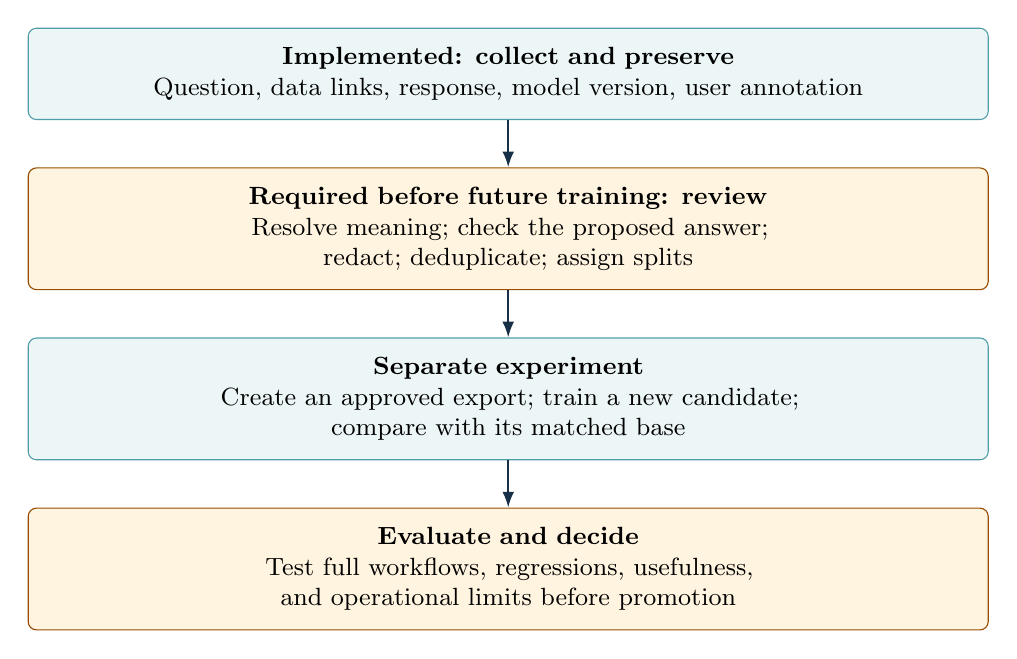
\begin{tikzpicture}[node distance=6mm]
\node[box,text width=11.7cm] (collect)
{\textbf{Implemented: collect and preserve}\\Question, data links, response, model version, user annotation};
\node[gate,text width=11.7cm,below=of collect] (review)
{\textbf{Required before future training: review}\\Resolve meaning; check the proposed answer;\\redact; deduplicate; assign splits};
\node[box,text width=11.7cm,below=of review] (learn)
{\textbf{Separate experiment}\\Create an approved export; train a new candidate;\\compare with its matched base};
\node[gate,text width=11.7cm,below=of learn] (evaluate)
{\textbf{Evaluate and decide}\\Test full workflows, regressions, usefulness,\\and operational limits before promotion};
\draw[arrow] (collect) -- (review);
\draw[arrow] (review) -- (learn);
\draw[arrow] (learn) -- (evaluate);
\end{tikzpicture}
\caption{The intended feedback-to-improvement loop. Collection exists now.
Automatic training from newly collected pilot annotations is not implemented
or enabled by the completed adapter runs.}
\end{figure}

\section{What still limits the system}

\subsection{Semantic coverage and model generalization}
The toolkit supports a defined portfolio, with restrictions on weights,
direction, and temporal patterns. A capable language model cannot create a
missing implementation by describing one. Within the portfolio, the account
grouping regression shows that semantically close operations remain difficult.
Training on synthetic cards and related phrasing has not established reliable
interpretation of arbitrary business questions.

\subsection{Evaluation and data limitations}
The evaluation questions, small graphs, and oracles were designed for development.
Original wording overlap, later grading changes, and label audits are material
limitations. The public-data samples were small and selected for exact checking,
not representative of full workplace, biological, or transport datasets. A
reserved source can reduce one kind of development leakage, but it cannot prove
that the pretrained model has never encountered similar data or tasks.

\subsection{Performance and operations}
No general GPU speedup, concurrent-user throughput, or large-graph capacity claim
is established by the pilot acceptance. Enumerating groups can create a large
output even when the graph fits in memory. The browser and model receive bounded
views, so truncation and partial materialization must be visible. GPU 1 also
holds the router, reducing the memory available for native work. The serial
worker limits simultaneous native jobs but is not a complete multi-user
resource scheduler.

\subsection{Access and persistence}
The pilot uses a shared API token and a shared workspace. Request validation
checks session/file consistency, but that does not provide per-user account
isolation: people with the shared credential are not separate security tenants.
The pilot also saves conversations and uploaded data for review. Expanding to
external users requires explicit choices about access, retention, deletion,
consent, and which evidence may enter a training dataset.

The installation has since been stopped at the user's request. API and router
automatic startup are disabled, and the FP8 server is stopped. This document
describes the installed implementation and recorded acceptance, not a claim
that an endpoint is presently running.

\section{A concrete next research phase}

The next phase should turn observed user difficulties into testable changes.
The following are proposed work, not results already achieved:

\begin{enumerate}
\item \textbf{Repair grouping semantics.} Build contrasting practical requests
  for full groups, the largest group, and all fixed-size groups; independently
  check the labels and replay the known payment failure.
\item \textbf{Finish the pending comparisons.} Complete matched business
  workflows, retention checks, and real-data comparisons before using the
  untouched reserved source for a declared final protocol.
\item \textbf{Collect actual user questions.} Measure clarification usefulness,
  task completion, and comprehension of names, tables, and visualizations.
  Keep assistant-authored acceptance feedback separately labeled.
\item \textbf{Review before training.} Produce a curated candidate dataset with
  source provenance and conversation/source-level split boundaries. Keep raw
  annotations and reviewed targets as distinct artifacts.
\item \textbf{Attribute improvements.} Compare model updates against the same
  base/runtime; evaluate code and UI changes separately where possible. Include
  multiple runs or seeds and uncertainty estimates appropriate to correlated cases.
\item \textbf{Measure deployment limits.} Test realistic graph sizes, result
  volumes, GPU sharing, and concurrent requests. Add account-level controls
  before treating the shared pilot as a multi-tenant product.
\end{enumerate}

The research question is whether the complete system helps people obtain the
right analysis from their own language and data. The present evidence supports
a working integration and a limited routing improvement. Answering that broader
question requires the application and user evaluations above.

\appendix
\clearpage
\section{Reproduction and evidence map}

All paths in this appendix are relative to the repository root. The source
snapshot has substantial existing uncommitted work; a Git revision alone would
not identify every file described here. The companion
\pathref{evidence_manifest.json} records SHA-256 hashes of selected source and
report files read for this note. It is an index of evidence, not a new run of the
experiments. No private API token or user conversation is embedded in the paper.

\subsection{Implementation entry points}

\begin{longtable}{@{}P{0.57\linewidth}P{0.39\linewidth}@{}}
\toprule
File or directory & Role \\
\midrule
\endhead
\pathref{graphmine_catalog.json} & Formal problems, support boundary, and backend
provenance. \\
\pathref{graphmine_manifest.json} & Compact operation and CLI contract. \\
\pathref{library/} & C++/CUDA interfaces, adapters, native CLI, and tests. \\
\pathref{agent/graphmine_agent/models.py} & Typed routing, planning, result, and
feedback contracts. \\
\pathref{agent/graphmine_agent/agent_service.py} & Conversation stages and
orchestration. \\
\pathref{agent/graphmine_agent/graph_store.py}\newline
\pathref{agent/graphmine_agent/graph_context.py} & Ingestion, data context,
inspection, and projections. \\
\pathref{agent/graphmine_agent/planning.py}\newline
\pathref{agent/graphmine_agent/execution.py} & Validation and native execution. \\
\pathref{agent/graphmine_agent/selector.py} & Deterministic backend selection. \\
\pathref{agent/graphmine_agent/answers.py}\newline
\pathref{agent/graphmine_agent/presentation.py} & Facts, source-record joins,
tables, and follow-up choices. \\
\pathref{agent/graphmine_agent/adapter_server.py} & Pinned business router service. \\
\pathref{agent/graphmine_agent/learning/finetune.py} & Token masking, adapter
training, checkpoints, and status. \\
\pathref{agent/graphmine_agent/learning/business_curriculum.py}\newline
\pathref{agent/graphmine_agent/learning/oracles.py} & Business export and independent
bounded answer checks. \\
\pathref{agent/graphmine_agent/learning/adapter_eval.py}\newline
\pathref{agent/graphmine_agent/learning/adapter_workflows.py} & Matched static routing
and conversation runtimes. \\
\pathref{agent/graphmine_agent/commands.py}\newline
\pathref{agent/graphmine_agent/history.py} & Local commands and saved evidence. \\
\pathref{agent/graphmine_agent/static/} & Browser chat, results, and feedback UI. \\
\bottomrule
\end{longtable}

\subsection{Saved training artifacts}

The source curriculum and its native audit are
\pathref{.graphmine-learning/finetune-corpus-v2/} and
\pathref{.graphmine-learning/finetune-native-v1.json}. The practical curriculum
and exported supervision are
\pathref{.graphmine-learning/business-curriculum-v1/} and
\pathref{.graphmine-learning/business-routing-data-v1/}.

The completed run directories are
\pathref{.graphmine-learning/finetune-qwen27b-v3/} and
\pathref{.graphmine-learning/finetune-qwen27b-business-v1/}.
Each keeps \pathref{run.json}, \pathref{status.json}, \pathref{metrics.jsonl},
checkpoints, and final adapter files. The business base checkpoint revision is
\pathref{1d4bf0f2ff6012fd82039f2fa52739d0dd7c60c0}.
The business adapter SHA-256 is
\pathref{dd7017735094300c4a89f217cb094c0d8b9981d1c7d86182596a7a6f7ef5f4d6}.
The original adapter SHA-256 is
\pathref{276cfd92ab692442ead80bb0170af84860d0ce604f89b9bdf1fcacc152449b75}.

Recorded training package versions are PyTorch 2.13.0, Transformers 5.18.0,
PEFT 0.21.2, bitsandbytes 0.50.2, Accelerate 1.15.0, Datasets 5.0.1, and
flash-linear-attention 0.5.2. The matched evaluation adds XGrammar 0.2.8 and
apache-tvm-ffi 0.1.14.post1. These are observed environment pins, not a statement
that arbitrary newer versions produce equivalent results.

The routing service verifies the adapter fingerprint, training configuration,
base files, runtime prompt, and response schema. The app verifies the router's
identity. If those checks fail, the intended behavior is a visible failure
rather than silently using a different routing model. Reproduction should retain
that binding between evaluated artifact and deployed artifact.

\section{Restarting the existing pilot}

Run these commands on the GPU server as the existing installation user.
They reuse the saved configuration, data, and weights. They do not resume
training or the stopped evaluation queue.

In terminal 1:
\begin{lstlisting}
cd /home/wajid/projects/graphDatabaseAgent/graphMine-repo
./deploy/start-vllm.sh
\end{lstlisting}
Keep the terminal open and wait for model startup to complete. In terminal 2:
\begin{lstlisting}
systemctl --user start graphmine-pilot-router.service graphmine-pilot-api.service
journalctl --user -u graphmine-pilot-router.service -u graphmine-pilot-api.service -f
\end{lstlisting}
Allow the router's weights to load. Open \url{http://127.0.0.1:18000} on the
server, or use its private network address from a connected computer. The existing
access token is \code{GRAPHMINE_API_TOKEN} in \pathref{agent/.env}; enter it in
the UI settings if prompted. Do not regenerate the environment merely to resume
the installation. The operator guide is \pathref{deploy/README.md}.

To stop the app and router:
\begin{lstlisting}
systemctl --user stop graphmine-pilot-api.service graphmine-pilot-router.service
\end{lstlisting}
Then press Ctrl+C in terminal 1 to stop vLLM. Closing the browser alone does not
stop the server processes.

\section{A compact glossary}

\begin{description}[style=nextline,leftmargin=1.5em,labelindent=0pt]
\item[Graph] Records represented as vertices and their relationships as edges.
\item[Routing] Selecting the intended analysis and expressing its requirements.
\item[Planning] Filling the selected operation's allowed settings and inputs.
\item[Backend] One native implementation of an operation.
\item[Schema constraint] A restriction on the structure of model output; it does
not guarantee the meaning is correct.
\item[Adapter] A saved set of learned parameter updates applied to a frozen base.
\item[Oracle] An independent reference calculation or check for a bounded test.
\item[Holdout] Data reserved from a specified development process. Its validity
depends on exactly which questions, graphs, and sources were kept separate.
\item[Grounded fact] A statement materialized from input records, validated plans,
or computation outputs, with a traceable source.
\item[Annotation] A saved user observation, correction, rating, or note awaiting
review before potential training use.
\end{description}

\begin{thebibliography}{99}
\small
\bibitem{lora}
Edward J. Hu et al.
\emph{LoRA: Low-Rank Adaptation of Large Language Models}. 2021.
\url{https://arxiv.org/abs/2106.09685}.

\bibitem{qlora}
Tim Dettmers, Artidoro Pagnoni, Ari Holtzman, and Luke Zettlemoyer.
\emph{QLoRA: Efficient Finetuning of Quantized LLMs}. 2023.
\url{https://arxiv.org/abs/2305.14314}.

\bibitem{implementation}
GraphMine project. Application implementation and user guide.
\pathref{agent/graphmine_agent/}; \pathref{agent/README.md}.
Local working-tree snapshot, October 2026.

\bibitem{catalog}
GraphMine project. Formal problem catalog and runtime manifest.
\pathref{graphmine_catalog.json}; \pathref{graphmine_manifest.json}.

\bibitem{release}
GraphMine project. Recorded V1 release scope and acceptance.
\pathref{docs/V1.md}. The acceptance snapshot is dated 1 October 2026.

\bibitem{training}
GraphMine project. Training implementation and saved run configuration.
\pathref{agent/graphmine_agent/learning/finetune.py};
\pathref{.graphmine-learning/finetune-qwen27b-business-v1/run.json};
\pathref{.graphmine-learning/finetune-qwen27b-business-v1/status.json}.

\bibitem{completion}
GraphMine project. Completed adapter verification records.
\pathref{agent/evaluation/reports/finetune-completion-2026-10-03.json};
\pathref{agent/evaluation/reports/business-finetune-completion-2026-10-03.json}.

\bibitem{curriculum}
GraphMine project. Business-question curriculum record.
\pathref{agent/evaluation/reports/business-question-curriculum-2026-10-03.json};
\pathref{.graphmine-learning/business-curriculum-v1/manifest.json}.
Distinct-question counts are also recorded in the stop/handoff report.

\bibitem{progress}
GraphMine project. Development and training history.
\pathref{agent/IMPROVEMENT_PLAN.md};
\pathref{agent/evaluation/FINETUNING_PROGRESS.md}.
Historical milestones must be read with their dates and later updates.

\bibitem{originaleval}
GraphMine project. Original 132-case routing comparison and review.
\pathref{agent/evaluation/reports/adapter-test-review-2026-10-03.json}.

\bibitem{challenge}
GraphMine project. Challenge review, including audited label results.
\pathref{agent/evaluation/reports/adapter-challenge-review-2026-10-03.json}.

\bibitem{workflow}
GraphMine project. Original adapter application comparisons.
\pathref{agent/evaluation/reports/adapter-workflow-comparison-2026-10-03.json};
\pathref{agent/evaluation/reports/adapter-realworld-comparison-2026-10-03.json}.

\bibitem{numericaudit}
GraphMine project. Numeric-filter grading addendum.
\pathref{agent/evaluation/reports/adapter-realworld-numeric-filter-audit-2026-10-03.json}.

\bibitem{businesseval}
GraphMine project. Business routing comparison and serving reference.
\pathref{agent/evaluation/reports/adapter-business-new-review-v1.json};
\pathref{agent/evaluation/reports/adapter-business-fp8-review-2026-10-03.json}.

\bibitem{changeaudit}
GraphMine project. Paired business-route change audit.
\pathref{agent/evaluation/reports/business-routing-change-audit-v1.json}.

\bibitem{regression}
GraphMine project. Saved-route payment-group diagnostic.
\pathref{agent/evaluation/reports/business-payment-regression-replay-v1.json}.

\bibitem{stoprecord}
GraphMine project. Fine-tuning stop and handoff.
\pathref{agent/evaluation/reports/finetuning-user-stop-2026-10-03.json}.

\bibitem{deployment}
GraphMine project. Pilot integration and acceptance record.
\pathref{agent/evaluation/reports/pilot-deployment-2026-10-04.json}.
Later operational shutdown and restart instructions are in
\pathref{deploy/README.md}.

\bibitem{feedback}
GraphMine project. Local commands, annotation storage, and export implementation.
\pathref{agent/graphmine_agent/commands.py};
\pathref{agent/graphmine_agent/database.py};
\pathref{agent/graphmine_agent/history.py};
\pathref{agent/graphmine_agent/api.py}.
\end{thebibliography}

\end{document}
